\documentclass[handout]{beamer}
\usetheme[faculty=science, university=uu, logo=uu-logo]{fibeamer}
\usepackage[utf8]{inputenc}
\usepackage[main=english]{babel}        %% typeset as follows:
\title{On modelling the Earth} %% that will be typeset on the
%\subtitle{Presentation Subtitle} %% title page.
\author{c.thieulot@uu.nl}
%% These additional packages are used within the document:
\usepackage{ragged2e}  % `\justifying` text
\usepackage{booktabs}  % Tables
\usepackage{tabularx}
\usepackage{tikz}      % Diagrams
\usetikzlibrary{calc, shapes, backgrounds}
\usepackage{amsmath, amssymb}
\usepackage{url}       % `\url`s
\usepackage{listings}  % Code listings
\frenchspacing

%%%%%%%%%%%%%%%%%%%%%%%%%%%%%%%%%%%%%%%%%%%%%%%%%%%%%%%%%%%%%%%%%%%%%%%%%%%%%%%%%%%%%%%%%%%%%%%%%%%%%5
\begin{document}
  \frame{\maketitle}

  \AtBeginSection[]{% Print an outline at the beginning of sections
    \begin{frame}<beamer>
      \frametitle{Outline for Section \thesection}
      \tableofcontents[currentsection]
    \end{frame}}


\section{Planet Earth}

\begin{frame}[plain]{}
\includegraphics[width=1.\textwidth]{images/planet}\\
$\sim4.54 \cdot 10^9$ years old
\hspace{4.5cm}
$\sim 6\cdot10^{24}$ kg
\end{frame}

%------------------------------------------------------------------------------
\begin{frame}[plain]{The Earth (1)}
\begin{columns}[onlytextwidth]
\column{.45\textwidth}
\includegraphics[width=1.\textwidth]{images/shape}\\
$\delta R/R \simeq 0.3\%$
\column{.5\textwidth}
Plate tectonics theory:\\
\includegraphics[width=1.\textwidth]{images/plates}\\
\includegraphics[width=0.32\textwidth]{images/rift}
\includegraphics[width=0.32\textwidth]{images/subd}
\includegraphics[width=0.32\textwidth]{images/transf}
\end{columns}
\end{frame}

%------------------------------------------------------------------------------
\begin{frame}[plain]{The Earth (2)}
\begin{columns}[onlytextwidth]
\column{.5\textwidth}
\includegraphics[width=1.\textwidth]{images/earth}
\column{.45\textwidth}
The solid earth interacts with:
\begin{itemize}
\item the hydrosphere
\item the atmosphere
\item the biosphere
\end{itemize}
\end{columns}
\end{frame}

%------------------------------------------------------------------------------
\begin{frame}[plain]{The Earth (3)}
\begin{columns}[onlytextwidth]
\column{.5\textwidth}
\includegraphics[width=1.\textwidth]{images/history}
\column{.5\textwidth}
\includegraphics[width=1.\textwidth]{images/tronnes}\\
{\tiny [Trønnes, Mineral. Petrol., 2010]}
\end{columns}
\end{frame}

%------------------------------------------------------------------------------
\begin{frame}[plain]{The Earth (4)}

\begin{itemize}
\item Complex dynamical system $\rightarrow$ I will focus on the Solid Earth.
\pause
\item Maxwell relaxation time: $t_M = \eta/\mu \simeq 10^3yr$.
Elastic behaviour can be neglected when studying phenomena taking place at Myr scale 
(e.g. mantle convection) but not for short phenomena (e.g. Earthquakes, glacial rebound).  REFFFF
\pause
\item Reynold's number $Re=\rho u L/\eta \sim 10^{-20}$ $\rightarrow$ inertia negligeable
\end{itemize}

\vspace{.3cm} 
\pause

{\it "It is no exaggeration to say that the theory of slow viscous flow is the very heart of geodynamics."}
Neil Ribe, 2018.

%Slow viscous flow $\rightarrow$ Stokes equations.
\end{frame}

%------------------------------------------------------------------------------
\begin{frame}[plain]{The Earth (5)}

Earth is a heat engine: 
internal heat is a combination of residual heat from planetary accretion ($\sim$20\%) 
and radioactive decay ($\sim$80\%). 
\begin{center}
\includegraphics[height=2.65cm]{images/tempprofile}
\includegraphics[height=2.65cm]{images/thermalbig}
\includegraphics[height=2.65cm]{images/slide1} \\
\includegraphics[width=0.7\textwidth]{images/heatflux_mod} 
\end{center}

\end{frame}

%------------------------------------------------------------------------------
\begin{frame}[plain]{The Earth (6)}

\begin{center}

\includegraphics[height=2cm]{images/minion}

I need to solve the\\
{\bf mass}, {\bf momentum}, {\bf energy}\\
conservation equations for Stokes flow

\pause

+

additional (geo)physics ?

\end{center}

%\includegraphics[width=0.8\textwidth]{images/eqs}\\
%{\tiny (ASPECT code manual)}

\end{frame}

%------------------------------------------------------------------------------
\begin{frame}[plain]{The Earth (7)}

\begin{center}
\includegraphics[height=2.75cm]{images/RadialDensityPREM_mod}
\end{center}
\vspace{-0.5cm}
\begin{itemize}
\item Outer Core viscosity $\sim 1$Pa.s but mantle viscosity $\eta_m > 10^{21}$Pa.s \\
$\rightarrow$ core dynamics inaccessible to solid Earth modellers.

\pause

\item {\bf simple}: Earth is a giant Rayleigh-B{\'e}nard experiment in a perfectly spherical hollow sphere
with

\[
Ra= \frac{\rho_0^2 \alpha \Delta T D^3 g C_p }{\eta k} \sim 10^6 - 10^8 >>  Ra_c
\]

\end{itemize}

\end{frame}


%------------------------------------------------------------------------------
\begin{frame}[plain]{The Earth (7)}

\begin{center}
\includegraphics[width=0.56\textwidth]{images/x-movie0700}\\
{\tiny \url{https://youtu.be/j63MkEc0RRw}}
\end{center}
\end{frame}

%------------------------------------------------------------------------------
\begin{frame}[plain]{The Earth (7)}

\begin{center}
\includegraphics[width=0.22\textwidth]{images/stick}\\
Wait a second ... ?
\end{center}

\end{frame}


\section{Rheology}

%------------------------------------------------------------------------------
\begin{frame}[plain]{Rheology (1)}

What is the rheology of the fluid(s)?\\ \pause
What are the mantle and the crust made of?

\pause
 
\begin{itemize}
\item mantle is  45\% O, 22\% Si, and 23\% Mg (+ Fe, Al, Ca, Na, K)
\item These elements are all bound together in the form of silicate rocks (e.g. olivine, pyroxenes, spinel, and garnet).
\item These rocks are subjected to large $\Delta T$ ($10^3$K) and $\Delta P$ ($10^{10}$Pa).
\item Long time scales: viscous flow
\item They have undergone 4Byr of deformation (mix? anisotropy?)
\item They contain water (or not? how much? where?)
\item The mineral grain size changes  
\end{itemize}

\end{frame}

%------------------------------------------------------------------------------
\begin{frame}[plain]{Rheology (1)}


\begin{center}
\includegraphics[width=0.3\textwidth]{images/picrite} \hspace{1.5cm}
\includegraphics[width=0.34\textwidth]{images/garnet_peridotite_wehrlite} \\
{\tiny Phenocrysts in ultramafic picritic rock, 5cm \hspace{1cm}
Olivine with pyrope and chromian diopside in peridotite, 25cm} \\
\includegraphics[width=0.34\textwidth]{images/olivine_basalt_Oahu} \hspace{1cm}
\includegraphics[width=0.3\textwidth]{images/dunite_with_chlorite11cm} \\
{\tiny Basalt or picrite with olivine 6cm  \hspace{1cm}
Dunite with dark green chlorite, 11cm}
\end{center}




\end{frame}


%------------------------------------------------------------------------------
\begin{frame}[plain]{Rheology (2)}

Welcome to the fun world of geochemistry/petrology!

\vspace{.4cm}

\begin{columns}[onlytextwidth]
\column{.47\textwidth}
{\tiny The three-component chemical system MgO-Al$_2$O$_3$-SiO$_2$ (MAS) accounts for 89\% of the Earth’s mantle.}\\
\includegraphics[width=0.85\textwidth]{images/masliquidus}\\
{\tiny The system $MgO-Al_2O_3-SiO_2$ at 1 atm. pressure} %Diagram shows temperature contours and liquidus surface.  
\column{.5\textwidth}
\includegraphics[width=0.85\textwidth]{images/olivine}\\
{\tiny [Christensen, Annu. Rev. Earth Planet Sci. 1995]}
\end{columns}

\end{frame}


%------------------------------------------------------------------------------
\begin{frame}[plain]{Rheology (3) - ductile regime}

\begin{columns}[onlytextwidth]
\column{.45\textwidth}
Lab experiments
\includegraphics[width=0.95\textwidth]{images/hpt1}\\
{\tiny Triaxial compression apparatus (Utrecht Univ.)\\
confining press. up to 100 MPa, 
temp. up to $400^o$ C, constant strain rate (10$^{-4}$-10$^{-7}$ s$^{-1}$).} 
\pause
\column{.5\textwidth}
\includegraphics[width=0.95\textwidth]{images/kara10_mod}\\
{\tiny (valid for P=7GPa, T=1700K)}\\
%Gibbs energy minimisation software\\
%PerpleX, Burnman 
\end{columns}

\vspace{.4cm}
\[
\dot\varepsilon = A \left(\frac{\sigma}{\mu}\right)^n \left(\frac{b}{d}\right)^m \exp\left( -\frac{Q+pV}{RT} \right)
\]
{\tiny [Karato \& Wu, Science, 1993]}

\end{frame}

%------------------------------------------------------------------------------
\begin{frame}[plain]{Rheology (3) - ductile regime}

\begin{columns}[onlytextwidth]
\column{.5\textwidth}
Different labs:\\
\includegraphics[width=0.95\textwidth]{images/viscpb1_mod}\\
{\tiny upper mantle with a typical oceanic
geotherm calculated from the power-law creep const. relationship for olivine}
\column{.5\textwidth}
Water content\\
\includegraphics[width=0.95\textwidth]{images/viscpb2_mod}\\
{\tiny The influence of water depletion on viscosity (at 200 km depth: P = 7 GPa,
T = 1700 K, = 0.1 MPa)}
\end{columns}

\end{frame}

%------------------------------------------------------------------------------
\begin{frame}[plain]{Rheology (4) - brittle regime}

\begin{columns}[onlytextwidth]
\column{.5\textwidth}
When stress reaches the yield value, the rock breaks:\\
\includegraphics[width=.8\textwidth]{images/fossen}
\pause
\column{.5\textwidth}
\includegraphics[width=.8\textwidth]{images/buwa06a}\\
\includegraphics[width=1\textwidth]{images/buwa06b}
\end{columns}

Viscous-plastic rheologies

faults = high deformation rate zones of narrow width. 

 {\tiny [Duretz et al, G3, 2018; Spiegelman et al, G3, 2016; Thieulot at al, in prep.]} 

\end{frame}


%------------------------------------------------------------------------------
\begin{frame}[plain]{Rheology (5) - Putting it all together}
\begin{columns}[onlytextwidth]
\column{.35\textwidth}
\includegraphics[width=1\textwidth]{images/wabj08d}\\
\includegraphics[width=1.05\textwidth]{images/wabj08c}\\
\includegraphics[width=1.05\textwidth]{images/wabj08b}
\column{.65\textwidth}
\pause
\includegraphics[width=1\textwidth]{images/wabj08a}
\end{columns}
\end{frame}

%------------------------------------------------------------------------------
\begin{frame}[plain]{Rheology (5) - Putting it all together}
\begin{columns}[onlytextwidth]
\column{.35\textwidth}
\includegraphics[width=1\textwidth]{images/wabj08d}\\
\includegraphics[width=1.05\textwidth]{images/wabj08c}\\
\includegraphics[width=1.05\textwidth]{images/wabj08b}
\column{.65\textwidth}
\includegraphics[width=1\textwidth]{images/wabj08a_frame}
\end{columns}
\end{frame}




%------------------------------------------------------------------------------
\begin{frame}[plain]{Rheology (5) - Putting it all together}
\includegraphics[width=0.8\textwidth]{images/gltu95}
\pause
\[
\dot\varepsilon = A \left(\frac{\sigma}{\mu}\right)^n \left(\frac{b}{d}\right)^m \exp\left( -\frac{Q+pV}{RT} \right)
\]
\end{frame}



\section{Modelling}

%------------------------------------------------------------------------------
\begin{frame}[plain]{Analogue modelling (1)}

\includegraphics[width=0.6\textwidth]{images/anal1}

\includegraphics[width=0.8\textwidth]{images/anal6}

%analogue viscous materials: honey, silicon putty

%analogue brittle materials: sand, glass powders



\end{frame}

%------------------------------------------------------------------------------
\begin{frame}[plain]{Analogue modelling (2)}

\includegraphics[width=0.45\textwidth]{images/anal4}
\includegraphics[width=0.45\textwidth]{images/piv}

\includegraphics[width=0.45\textwidth]{images/anal2}
\includegraphics[width=0.45\textwidth]{images/anal3}

{\tiny [Koyi, Journal of Petroleum Geology, 1997; Schellart \& Strak, J. of Geodyn., 2016]}

\end{frame}

%------------------------------------------------------------------------------
\begin{frame}[plain]{Analogue modelling (3)}

'easy' to change density \& viscosity, geometries, but gravity?

\pause 

\includegraphics[width=0.72\textwidth]{images/cort08}

{\tiny [Corti, Nature Geo, 2008]}

\end{frame}



%------------------------------------------------------------------------------
\begin{frame}[plain]{Analogue modelling (4)}

\begin{center}
\includegraphics[width=0.25\textwidth]{images/dagm13a}
\includegraphics[width=0.35\textwidth]{images/dagm13b}
\end{center}
\vspace{-.4cm}
Herschel-Bulkley fluid (carbopol) is seeded with three types of encapsulated thermo-chromic 
liquid crystals (TLC), each reflecting light at a different temperature.

{\tiny [Davaille et al, J. of Non-Newtonian Mech., 2013] - Lab. FAST, Univ. Paris Sud}

\end{frame}

%------------------------------------------------------------------------------
\begin{frame}[plain]{Analogue vs Numerical ?}

\begin{columns}[onlytextwidth]
\column{.5\textwidth}
\includegraphics[width=0.85\textwidth]{images/madd13}\\
{\tiny [Massmeyer et al, J. of Non-Newtonian Mech., 2013]}
\column{.5\textwidth}
\includegraphics[width=0.95\textwidth]{images/bube06}\\
{\tiny [Buiter et al, Geological Society London, 2006]}
\end{columns}

\end{frame}

%------------------------------------------------------------------------------
\begin{frame}[plain]{Computational geodynamics}

What the community needs:
\begin{itemize}
\item open-source, well documented \& tested code (+ community)
\item flexible physics/numerics
\item state-of-the-art numerical methods
\item massively parallel
\pause
\item capable to handle large viscosity contrasts
\end{itemize}

\includegraphics[width=6cm]{images/vava08_mod}
\includegraphics[width=6cm]{images/thie11_mod}

%\pause

%70's, 80's: spectral methods, stream function. Now: FDM, FEM, FVM.


\end{frame}

%------------------------------------------------------------------------------
\begin{frame}[plain]{Computational geodynamics - ASPECT }
\begin{columns}[onlytextwidth]
\column{.5\textwidth}
\includegraphics[width=3.75cm]{images/manual}\\
{\tiny \url{https://github.com/geodynamics/aspect}}\\
{\tiny \url{https://geodynamics.org/cig/software/aspect/}}\\
{\tiny \url{https://www.dealii.org/}}
\column{.5\textwidth}
\begin{itemize}
\item developed on deal.ii (FE library, 20+ years existence)\\
\includegraphics[width=3cm]{images/dealii}
\item 600+ tests
\item 550+ page up-to-date manual (doxygen)
\item community (hackathons)\\
\includegraphics[width=3cm]{images/groupphoto}
\end{itemize}
\end{columns}
\end{frame}

%------------------------------------------------------------------------------
\begin{frame}[plain]{Computational geodynamics - ASPECT features}

\begin{columns}[onlytextwidth]
\column{.6\textwidth}

C++

2D/3D

Compressible \& incompressible flow

Cartesian \& Spherical geometries

FEM (deal.ii) ($Q_2\times Q_1$ or $Q_2\times P_{-1}$)

Trilinos (or PetSc) parallel iterative solver

Adaptive mesh refinement AMR (p4est)

Extensive benchmarking\\
{\tiny [Kronbichler et al, GJI, 2012; Tosi et al, G3, 2015; Dannberg \& Heister, GJI, 2016; Heister et al, GJI, 2017; Thieulot, S.E. 2017; Glerum et al, SE, 2018; Liu \& King, GJI, 2019]}\\
{\tiny\url{http://www.p4est.org/}, \url{https://trilinos.github.io/}}

\column{.5\textwidth}

\includegraphics[width=4cm]{images/annesubd}\\
{\tiny [Glerum et al., SE, 2018]}

\end{columns}
\end{frame}


%------------------------------------------------------------------------------
\begin{frame}[plain]{Computational geodynamics - Numerical algor.}

\[
\left(
\begin{array}{cc}
A & B^T \\
B & 0 
\end{array}
\right)\cdot
\left(
\begin{array}{c}
{\cal V} \\ {\cal P}
\end{array}
\right)
=
\left(
\begin{array}{cc}
f \\ g
\end{array}
\right)
\]
Stokes system $\rightarrow$ saddle point problem solved with FGMRES. 

\pause

Preconditioner 
\[
P = 
\left(
\begin{array}{cc}
\widetilde{A^{-1}} & -\widetilde{A^{-1}} B^T \widetilde{S^{-1}}\\ 
0 & \widetilde{S^{-1}}
\end{array}
\right)
\]
where $\widetilde{A^{-1}}$, $\widetilde{S^{-1}}$ approximate the exact inverses. 

\begin{itemize}
\item $\widetilde{A^{-1}}$: CG (loose tol ), precond with AMG (and now GMG)
\item $\widetilde{S^{-1}}$: inverse of the Schur complement matrix $S=BA^{-1}B^T$ approx. by the inv. of 
a (weighted) mass matrix in press. space
\end{itemize}

{\tiny [Geenen et al, G3, 2009; ur Rehman et al, IJNMF, 2011; Kronbichler et al, GJI, 2012; Clevenger et al, subm.]}
\end{frame}



%------------------------------------------------------------------------------
\begin{frame}[plain]{Computational geodynamics - Numerical algor.}

Energy equation (Temperature): advection-diffusion equation with high Peclet number
\[
Pe=h |v| / \kappa \sim 10^{2}-10^4
\]

\begin{itemize}
\item advection is stabilised:  
Entropy stabilisation {\tiny [Guermond et al, JCP, 2011]} or SUPG {\tiny [Brooks \& Hughes, CMAME, 1982]} 
\item 
time discretisation: second-order
accurate implicit/explicit time stepping scheme based on the BDF-2 scheme {\tiny [Hairer \& Wanner, 1991]}
\end{itemize} 


{\tiny [Kronbichler et al, GJI, 2012]}
\end{frame}

%------------------------------------------------------------------------------
\begin{frame}[plain]{Computational geodynamics - Material tracking}

\begin{center}
\includegraphics[width=2.97cm]{images/diapirs0010.png}
\includegraphics[width=2.97cm]{images/diapirs0015.png} {\tiny [Louis-Napoleon et al, in prep.]}
\end{center}

\pause

\begin{itemize}
\item
Field based method ("compositions") {\tiny [Kronbichler, GJI, 2012]}

\item
Discontinuous Galerkin (+BPL) {\tiny [He et al, PEPI, 2017]}

\item
Volume of Fluid {\tiny [Puckett et al, PEPI, 2018]}

\item
Marker-in-cell {\tiny [Gassmoeller et al, G3, 2018; GJI, 2019]}\\
\includegraphics[width=4cm]{images/galh18}
\end{itemize}

\pause
also Level Set {\tiny [Bourgouin et al, GJI, 2007; Braun et al, PEPI, 2008; Samuel \& Evonuk, G3, 2010]}
\end{frame}


%------------------------------------------------------------------------------
\begin{frame}[plain]{The Earth (6)}

\begin{center}
\includegraphics[height=2cm]{images/minion}

I need to solve the\\
{\bf mass}, {\bf momentum}, {\bf energy}\\
conservation equations for Stokes flow

+

additional (geo)physics ?

\end{center}

%\includegraphics[width=0.8\textwidth]{images/eqs}\\
%{\tiny (ASPECT code manual)}

\end{frame}



%------------------------------------------------------------------------------
\begin{frame}[plain]{Computational geodynamics - Melt}

\begin{columns}[onlytextwidth]
\column{.5\textwidth}
\includegraphics[width=5cm]{images/dahe16a}
\includegraphics[width=5cm]{images/dahe16b}

\column{.5\textwidth}
\includegraphics[width=4.5cm]{images/daga18a}
\includegraphics[width=4.5cm]{images/daga18b}
\end{columns}

\vspace{3mm}

{\tiny [Gerya \& Meilick, JMG, 2011; Keller et al, GJI, 2013; Bouilhol et al, EPSL, 2005; ...]}
\end{frame}

%------------------------------------------------------------------------------
\begin{frame}[plain]{Computational geodynamics - More!}

\begin{itemize}

\item 
Grain-size evolution\\
\frame{\includegraphics[height=1cm]{images/daef17}
\includegraphics[height=1cm]{images/daef17b}}\\
{\tiny [Solomatov, EPSL, 2001, Cerpa et al, JGR, 2017]}

\item 
Coupling with surface processes (paleo-climate)\\
\frame{\includegraphics[height=1cm]{images/brya10}
\includegraphics[height=1cm]{images/uewg15}}\\
{\tiny [Braun \& Yamato, Tect., 2010; Braun \& Willett, Geomorph., 2013; Thieulot et al, G3, 2014, Ueda et al, Tect., 2015]}

\item 
PDEs are highly nonlinear: taylored Newton solver 
\frame{\includegraphics[height=1cm]{images/frbt19}\includegraphics[height=1cm]{images/frbt19b}}

\item 
Seismo-thermo-poro-elasto-visco-plastic modelling\\
{\tiny [van Dinther et al, GRL, 2014; Gerya, 2018]} 

\end{itemize}

\end{frame}



\begin{frame}[plain]{Computational geodynamics - FEM + PETSc}
\begin{center}
\includegraphics[width=0.75\textwidth]{images/mabl15a}\\
\vspace{-2mm}
{\tiny Comput. Methods Appl. Mech. Engrg., 2015}\\
\includegraphics[height=3cm]{images/mabl15b}
\includegraphics[height=3cm]{images/mabl15c}
\end{center}

\vspace{-2mm}
Matrix-free operators reduce storage and memory bandwidth requirements
$\rightarrow$ improved speed and scalability on modern multi-core hardware. 

{\tiny [Le Pourhiet et al, EPSL, 2017; Jourdon et al, Terra Nova, 2018; EPSL, 2019]}
\end{frame}


\begin{frame}[plain]{Computational geodynamics - FDM + PETSc}

\begin{center}
\includegraphics[width=0.6\textwidth]{images/lamema}\\
\vspace{3mm}
\includegraphics[height=2.5cm]{images/lamemb}
\includegraphics[height=2.5cm]{images/lamemc}
\includegraphics[height=2.5cm]{images/lamemd}
\end{center}

{\tiny [Collignon et al, G3, 2014; Tectonophysics, 2015; Fernandez \& Kaus, GJI, 2015; Pusok et al, 2018]}

\end{frame}


%------------------------------------------------------------------------------
\begin{frame}[plain]{Computational geodynamics - FEM}

\includegraphics[width=0.75\textwidth]{images/algs}\\
200-300 million elements, 400-1200 Mdofs, 4000-5000 procs\\
+ inverse techniques
{\tiny [Stadler et al, Science, 2010; Alisic et al, JGR, 2012]}

\end{frame}

%------------------------------------------------------------------------------
\begin{frame}[plain]{Computational geodynamics - FVM}

\begin{center}
\includegraphics[width=0.75\textwidth]{images/coltice1}\\
Science Advances, 2019\\
\includegraphics[width=0.75\textwidth]{images/coltice2}\\
\includegraphics[width=0.85\textwidth]{images/coltice3}
\end{center}

{\tiny [Tackley, PEPI, 2008; Tackley, Earth Sc. Rev, 2012; ]}


\end{frame}




%------------------------------------------------------------------------------
\begin{frame}[plain]{Conclusions}

\begin{itemize}
\item Earth is fascinating object, but very complex
\item Analogue \& numerical modelling
\item Computational geodynamics benefits from state-of-the-art CFD 
\item Multi-physics: {\sl extremely} nonlinear coupled PDEs (strategy?)
\item Physical length-scale vs mesh resolution
\item Initial geometry and temperature field remain a problem
\end{itemize}

\pause

\begin{center}
Computational Geodynamics =\\ 
\includegraphics[height=1.5cm]{images/monsters}\hspace{.5cm} {\huge or}
\hspace{.5cm} \includegraphics[height=1.5cm]{images/science} ?
\end{center}

\end{frame}



%------------------------------------------------------------------------------
\begin{frame}[plain]{}\end{frame}
%------------------------------------------------------------------------------
\begin{frame}[plain]{}\end{frame}





%------------------------------------------------------------------------------
\begin{frame}[plain]{}
\includegraphics[height=2.5cm]{images/book1}
\includegraphics[height=2.5cm]{images/book2}
\includegraphics[height=2.5cm]{images/book3}
\includegraphics[height=2.5cm]{images/simpson}
\end{frame}

%------------------------------------------------------------------------------
\begin{frame}[plain]{}
\includegraphics[height=5cm]{images/kasa04}\\
{\tiny "Yin-Yang grid": An overset grid in spherical geometry, Kageyama \& Sato, G3, 2004}
\end{frame}




\end{document}







\begin{columns}[onlytextwidth]
\column{.5\textwidth}
\column{.5\textwidth}
\end{columns}



















%------------------------------------------------------------------------------
%------------------------------------------------------------------------------
    \subsection{Blind Text}
    \begin{frame}{Jabberwocky}
      \framesubtitle{Lewis Carroll}%
      \begin{tikzpicture}[overlay,remember picture]
        \node[anchor=south east,xshift=-30pt,yshift=35pt]
          at (current page.south east) {
            \includegraphics[width=35mm]{resources/jabberwocky-light}
          };
      \end{tikzpicture}%
      'Twas brillig, and the slithy toves\\
      Did gyre and gimble in the wabe;\\
      All mimsy were the borogoves,\\
      And the mome raths outgrabe.\\\bigskip

      “Beware the Jabberwock, my son!\\
      The jaws that bite, the claws that catch!\\
      Beware the Jubjub bird, and shun\\
      The frumious Bandersnatch!”\\
    \end{frame}

    \begin{frame}[label=lists]{Lists and locales}
      \framesubtitle{Lorem ipsum dolor sit amet}
      \begin{columns}[onlytextwidth]
        \column{.5\textwidth}
          \begin{itemize}
            \item Nulla nec lacinia odio. Curabitur urna tellus.
            \begin{itemize}
              \item Fusce id sodales dolor. Sed id metus dui.
              \begin{itemize}
                \item Cupio virtus licet mi vel feugiat.
              \end{itemize}
            \end{itemize}
          \end{itemize}
        \column{.5\textwidth}
          \begin{enumerate}
            \item Donec porta, risus porttitor egestas scelerisque video.
            \begin{enumerate}
              \item Nunc non ante fringilla, manus potentis cario.
              \begin{enumerate}
                \item Pellentesque servus morbi tristique.
              \end{enumerate}
            \end{enumerate}
          \end{enumerate}
      \end{columns}
      \bigskip
      \justifying

      {\uselanguage{czech}Nechť již hříšné saxofony ďáblů
      rozzvučí síň úděsnými tóny waltzu, tanga a quickstepu!}
      {\uselanguage{slovak} Nezvyčajné kŕdle šťastných figliarskych
      ďatľov učia pri kótovanom ústí Váhu mĺkveho koňa Waldemara
      obžierať väč\-šie kusy exkluzívnej kôry.}
      {\uselanguage{english}The quick, brown fox jumps over a lazy
      dog. DJs flock by when MTV ax quiz prog. “Now fax quiz Jack!”}
    \end{frame}

    \subsection{Structuring Elements}
    \begin{frame}[label=simmonshall]{Text blocks}
      \framesubtitle{In plain, example, and \alert{alert} flavour}
      \alert{This text} is highlighted.

      \begin{block}{A plain block}
        This is a plain block containing some \alert{highlighted text}.
      \end{block}
      \begin{exampleblock}{An example block}
        This is an example block containing some \alert{highlighted text}.
      \end{exampleblock}
      \begin{alertblock}{An alert block}
        This is an alert block containing some \alert{highlighted text}.
      \end{alertblock}
    \end{frame}

    \begin{frame}[label=proof]{Definitions, theorems, and proofs}
      \framesubtitle{All integers divide zero}
      \begin{definition}
        $\forall a,b\in\mathds{Z}: a\mid b\iff\exists c\in\mathds{Z}:a\cdot c=b$
      \end{definition}
      \begin{theorem}
        $\forall a\in\mathds{Z}: a\mid 0$
      \end{theorem}
      \begin{proof}[Proof\nopunct]
        $\forall a\in\mathds{Z}: a\cdot 0=0$
      \end{proof}
    \end{frame}

    \subsection{Numerals and Mathematics}
    \begin{frame}[label=math]{Numerals and Mathematics}
      \framesubtitle{Formulae, equations, and expressions}
      \begin{columns}[onlytextwidth]
        \column{.20\textwidth}
          1234567890
        \column{.20\textwidth}
          \oldstylenums{1234567890}
        \column{.20\textwidth}
          $\hat{x}$, $\check{x}$, $\tilde{a}$,
          $\bar{a}$, $\dot{y}$, $\ddot{y}$
        \column{.40\textwidth}
          $\int \!\! \int f(x,y,z)\,\mathsf{d}x\mathsf{d}y\mathsf{d}z$
      \end{columns}
      \begin{columns}[onlytextwidth]
        \column{.5\textwidth}
          $$\frac{1}{\displaystyle 1+
            \frac{1}{\displaystyle 2+
            \frac{1}{\displaystyle 3+x}}} +
            \frac{1}{1+\frac{1}{2+\frac{1}{3+x}}}$$
        \column{.5\textwidth}
          $$F:\left| \begin{array}{ccc}
          F''_{xx} & F''_{xy} &  F'_x \\
          F''_{yx} & F''_{yy} &  F'_y \\
          F'_x     & F'_y     & 0
          \end{array}\right| = 0$$
      \end{columns}
      \begin{columns}[onlytextwidth]
        \column{.3\textwidth}
          $$\mathop{\int \!\!\! \int}_{\mathbf{x} \in \mathds{R}^2}
          \! \langle \mathbf{x},\mathbf{y}\rangle\,\mathsf{d}\mathbf{x}$$
        \column{.33\textwidth}
          $$\overline{\overline{a\alpha}^2+\underline{b\beta}
           +\overline{\overline{d\delta}}}$$
        \column{.37\textwidth}
          $\left] 0,1\right[ + \lceil x \rfloor - \langle x,y\rangle$
      \end{columns}
      \begin{columns}[onlytextwidth]
        \column{.4\textwidth}
          \begin{eqnarray*}
           e^x &\approx& 1+x+x^2/2! + \\
             && {}+x^3/3! + x^4/4!
          \end{eqnarray*}
        \column{.6\textwidth}
          $${n+1\choose k} = {n\choose k} + {n \choose k-1}$$
      \end{columns}
    \end{frame}

    \subsection{Figures and Code Listings}
    \begin{frame}[label=figs1]{Figures}
      \framesubtitle{Tables, graphs, and images}
      \begin{table}[!b]
        {\carlitoTLF % Use monospaced lining figures
        \begin{tabularx}{\textwidth}{Xrrr}
          \textbf{Faculty} & \textbf{With \TeX} & \textbf{Total} &
          \textbf{\%} \\
          \toprule
          Faculty of Informatics       & 1\,716  & 2\,904  &
          59.09 \\% 1433
          Faculty of Science           & 786     & 5\,275  &
          14.90 \\% 1431
          Faculty of $\genfrac{}{}{0pt}{}{\textsf{Economics and}}{%
          \textsf{Administration}}$    & 64      & 4\,591  &
          1.39  \\% 1456
          Faculty of Arts              & 69      & 10\,000 &
          0.69  \\% 1421
          Faculty of Medicine          & 8       & 2\,014  &
          0.40  \\% 1411
          Faculty of Law               & 15      & 4\,824  &
          0.31  \\% 1422
          Faculty of Education         & 19      & 8\,219  &
          0.23  \\% 1441
          Faculty of Social Studies    & 12      & 5\,599  &
          0.21  \\% 1423
          Faculty of Sports Studies    & 3       & 2\,062  &
          0.15  \\% 1451
          \bottomrule
        \end{tabularx}}
        \caption{The distribution of theses written using \TeX\ during 2010--15 at MU}
      \end{table}
    \end{frame}
    \begin{frame}[label=figs2]{Figures}
      \framesubtitle{Tables, graphs, and images}
      \begin{figure}[b]
        \centering
        % Flipping a coin
        % Author: cis
        \tikzset{
          head/.style = {fill = none, label = center:\textsf{H}},
          tail/.style = {fill = none, label = center:\textsf{T}}}
        \scalebox{0.65}{\begin{tikzpicture}[
            scale = 1.5, transform shape, thick,
            every node/.style = {draw, circle, minimum size = 10mm},
            grow = down,  % alignment of characters
            level 1/.style = {sibling distance=3cm},
            level 2/.style = {sibling distance=4cm},
            level 3/.style = {sibling distance=2cm},
            level distance = 1.25cm
          ]
          \node[shape = rectangle,
            minimum width = 6cm, font = \sffamily] {Coin flipping}
          child { node[shape = circle split, draw, line width = 1pt,
                  minimum size = 10mm, inner sep = 0mm, rotate = 30] (Start)
                  { \rotatebox{-30}{H} \nodepart{lower} \rotatebox{-30}{T}}
           child {   node [head] (A) {}
             child { node [head] (B) {}}
             child { node [tail] (C) {}}
           }
           child {   node [tail] (D) {}
             child { node [head] (E) {}}
             child { node [tail] (F) {}}
           }
          };

          % Filling the root (Start)
          \begin{scope}[on background layer, rotate=30]
            \fill[head] (Start.base) ([xshift = 0mm]Start.east) arc (0:180:5mm)
              -- cycle;
            \fill[tail] (Start.base) ([xshift = 0pt]Start.west) arc (180:360:5mm)
              -- cycle;
          \end{scope}

          % Labels
          \begin{scope}[nodes = {draw = none}]
            \path (Start) -- (A) node [near start, left]  {$0.5$};
            \path (A)     -- (B) node [near start, left]  {$0.5$};
            \path (A)     -- (C) node [near start, right] {$0.5$};
            \path (Start) -- (D) node [near start, right] {$0.5$};
            \path (D)     -- (E) node [near start, left]  {$0.5$};
            \path (D)     -- (F) node [near start, right] {$0.5$};
            \begin{scope}[nodes = {below = 11pt}]
              \node [name = X] at (B) {$0.25$};
              \node            at (C) {$0.25$};
              \node [name = Y] at (E) {$0.25$};
              \node            at (F) {$0.25$};
            \end{scope}
          \end{scope}
        \end{tikzpicture}}
        \caption{Tree of probabilities -- Flipping a coin\footnote[frame]{%
          A derivative of a diagram from \url{texample.net} by cis, CC BY 2.5 licensed}}
      \end{figure}
    \end{frame}

    \defverbatim[colored]\sleepSort{
      \begin{lstlisting}[language=C,tabsize=2]
  #include <stdio.h>
  #include <unistd.h>
  #include <sys/types.h>
  #include <sys/wait.h>

  // This is a comment
  int main(int argc, char **argv)
  {
          while (--c > 1 && !fork());
          sleep(c = atoi(v[c]));
          printf("%d\n", c);
          wait(0);
          return 0;
  }
    \end{lstlisting}}
    \begin{frame}{Code listings}{An example source code in C}
      \sleepSort
    \end{frame}

    \subsection{Citations and Bibliography}
    \begin{frame}[label=citations]{Citations}
      \framesubtitle{\TeX, \LaTeX, and Beamer}

      \justifying\TeX\ is a programming language for the typesetting
      of documents. It was created by Donald Erwin Knuth in the late
      1970s and it is documented in \emph{The \TeX
      book}~\cite{knuth84}.

      In the early 1980s, Leslie Lamport created the initial version
      of \LaTeX, a high-level language on top of \TeX, which is
      documented in \emph{\LaTeX : A Document Preparation
      System}~\cite{lamport94}. There exists a healthy ecosystem of
      packages that extend the base functionality of \LaTeX;
      \emph{The \LaTeX\ Companion}~\cite{MG94} acts as a guide
      through the ecosystem.

      In 2003, Till Tantau created the initial version of Beamer, a
      \LaTeX\ package for the creation of presentations. Beamer is
      documented in the \emph{User's Guide to the Beamer
      Class}~\cite{tantau04}.
    \end{frame}

    \begin{frame}[label=bibliography]{Bibliography}
      \framesubtitle{\TeX, \LaTeX, and Beamer}
      \begin{thebibliography}{9}
        \bibitem{knuth84}
            Donald~E.~Knuth.
            \emph{The \TeX book}.
            Addison-Wesley, 1984.
        \bibitem{lamport94}
            Leslie~Lamport.
            \emph{\LaTeX : A Document Preparation System}.
            Addison-Wesley, 1986.
        \bibitem{MG94}
            M.~Goossens, F.~Mittelbach, and A.~Samarin.
            \emph{The \LaTeX\ Companion}.
            Addison-Wesley, 1994.
        \bibitem{tantau04}
            Till~Tantau.
            \emph{User's Guide to the Beamer Class Version 3.01}.
            Available at \url{http://latex-beamer.sourceforge.net}.
        \bibitem{MS05}
            A.~Mertz and W.~Slough.
            Edited by B.~Beeton and K.~Berry.
            \emph{Beamer by example} In TUGboat,
              Vol. 26, No. 1., pp. 68-73.
      \end{thebibliography}
    \end{frame}

\end{document}
